\section{Колебательный контур}

%Ижевск
\begin{ex}
\hspace{0pt} \\
\begin{minipage}{.65\textwidth}
Батарея из двух последовательных соединенных конденсаторов емкостью $C$ каждый заряжена до напряжения $U$ и в начальный момент времени подключена к катушке индуктивностью $L$, так что образовался колебательный контур. 
Спустя интервал времени $\tau$ один из конденсаторов пробивается, и сопротивление между обкладками становится равным нулю. 
Найдите амплитуду колебаний заряда на непробитом конденсаторе.
\end{minipage}
\begin{minipage}{.35\textwidth}
\centering
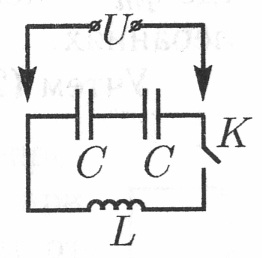
\includegraphics[width = 0.7 \textwidth]{1219OscillatoryCircuitCCL.jpg}
\end{minipage}
\begin{ans}
$q_{\max} = \frac{CU}{2}\sqrt{2-\cos^2 \left( \sqrt{\frac{2}{LC}} \tau \right)}$
\end{ans}
\end{ex}

%Кабардин-12.4
\begin{ex}
\hspace{0pt} \\
\begin{minipage}{.65\textwidth}
 Два конденсатора одинаковой электроемкости $C_1 = C_2 = C$ и катушка индуктивности $L$ соединены так, как показано на рисунке. 
В начальный момент времени ключ разомкнут, конденсатор $C_1$ заряжен до разности потенциалов $U$, а конденсатор $C_2$ не заряжен, 
сила тока в катушке равна нулю. Определите максимальное значение силы тока в катушке после замыкания цепи и период электромагнитных колебаний в цепи. 
\end{minipage}
\begin{minipage}{.35\textwidth}
\centering
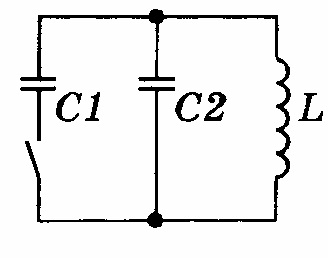
\includegraphics[width = 0.7 \textwidth]{1220OscillatoryCircuitC1C2L.jpg}
\end{minipage}
\begin{ans}
$I_{\max} = U \sqrt{\frac{C}{2L}}$, $T=2 \pi \sqrt{2LC}$
\end{ans}
\end{ex}

%Ижевск
\begin{ex}
\hspace{0pt} \\
\begin{minipage}{.65\textwidth}
В схеме, изображенной на рисунке, в некоторый момент времени замыкают ключ $K$, и конденсатор емкостью $C$, имеющий первоначальный заряд $q_0$, начинает заряжаться через катушку индуктивности $L$. 
Когда ток разряда достигает максимального значения, ключ $K$ вновь размыкают. Найти заряд $Q$, который протечет через резистор $R$. 
Сопротивление диода в прямом направлении много меньше $R$, в обратном - бесконечно велико.
\end{minipage}
\begin{minipage}{.35\textwidth}
\centering
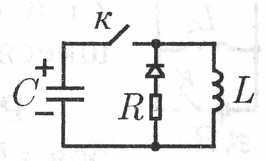
\includegraphics[width = 0.9 \textwidth]{1221OscillatoryCircuitCLR.jpg}
\end{minipage}
\begin{ans}
$q=\frac{q_0}{R}\sqrt{\frac{L}{C}}$
\end{ans}
\end{ex}

\begin{ex}
\hspace{0pt} \\
\begin{minipage}{.65\textwidth}
(2011) Электрический контур представляет собой треугольник, каждая сторона которого содержит емкость $C$, а вершины соединены с общей центральной точкой индуктивностями $L$. 
Пренебрегая сопротивлением и взаимной индуктивностью, найдите частоту возможных колебаний.
\end{minipage}
\begin{minipage}{.35\textwidth}
\centering
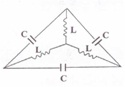
\includegraphics[width = 0.9 \textwidth]{122011OscillatoryCircuitTriangleCCCLLL.jpg}
\end{minipage}
\begin{ans}
\end{ans}
\end{ex}

\section{Переменный электрический ток}

%Ижевск
\begin{ex}
\hspace{0pt} \\
\begin{minipage}{.65\textwidth}
В изображенной на рисунке электрической цепи определите частоту приложенного переменного напряжения, при которой переменный ток через сопротивление не зависит от значения $R$. Индуктивность $L$ и емкость $C$ считать известными.
\end{minipage}
\begin{minipage}{.35\textwidth}
\centering
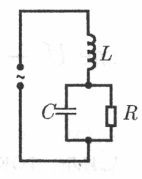
\includegraphics[width = 0.7 \textwidth]{1223AlternatingCurrentCLR.jpg}
\end{minipage}
\begin{ans}
$\omega = 1/\sqrt{LC}$
\end{ans}
\end{ex}

%Козел-10.5
\begin{ex}
\hspace{0pt} \\
\begin{minipage}{.65\textwidth}
В приведенной на рисунке схеме в момент $t$~=~0 замыкают ключ $K$. Найти зависимость от времени тока $I$, текущего через источник синусоидальной ЭДС $\mathcal{E}~=~\mathcal{E}_0 \sin \omega t$.
Параметры контура связаны соотношением $R\,=\,\sqrt{L/C}$.
\end{minipage}
\begin{minipage}{.35\textwidth}
\centering
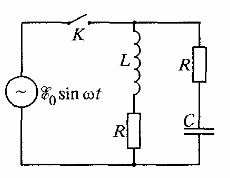
\includegraphics[width = 0.9 \textwidth]{1225AlternatingCurrentCLRR.jpg}
\end{minipage}
\begin{ans}
$I(t) = \frac{\mathcal{E}_0}{R} \sin \omega t$
\end{ans}
\end{ex}

%Козел-10.52
\begin{ex}
\hspace{0pt} \\
\begin{minipage}{.65\textwidth}
При каком условии амплитуда тока в цепи зависит только от амплитуды приложенного напряжения, но не от его частоты? Индуктивность $L$, и емкость $C$, и сопротивление $R$ считать известными.
\end{minipage}
\begin{minipage}{.35\textwidth}
\centering
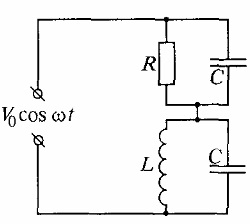
\includegraphics[width = 0.9 \textwidth]{1224AlternatingCurrentCCLR.jpg}
\end{minipage}
\begin{ans}
$L=R^2C$, $\tan \varphi = -\omega RC$
\end{ans}
\end{ex}